\documentclass[11pt]{article}
\usepackage{amsmath}
\usepackage{amsthm}
\usepackage{graphicx}
\usepackage{hyperref}
\usepackage[utf8]{inputenc}
\usepackage{enumitem}
\usepackage{cancel}
\usepackage{subcaption}
\usepackage{latexsym}
\usepackage{amsfonts}
\usepackage{bussproofs}
\usepackage{listings}
\usepackage{tikz}
\nocite{*}

\newcommand{\A}{{\mathbb{A}}}
\newcommand{\Evp}{{Ev (\bar{p})}}
\newcommand{\CTLf}{{CTL$^f$}}
\newcommand{\X}{{\mathbf{X}}}
\newcommand{\F}{{\mathbf{F}}}
\newcommand{\orr}{{\vee}}
\newcommand{\andd}{{\wedge}}
\newcommand{\phii}{{\varphi}}
\newcommand{\G}{{\mathbf{G}}}
\newcommand{\dia}{{\diamondsuit}}
\newcommand{\ARp}{{AR (p,\bot)}}
\def\CC{{C\nolinebreak[4]\hspace{-.05em}\raisebox{.4ex}{\tiny\bf ++}}}
\usepackage[a4paper, total={6in, 9in}]{geometry}

\bibliographystyle{plain}

\lstset{frame=tb,
  language=ML,
  aboveskip=3mm,
  belowskip=3mm,
  showstringspaces=false,
  columns=flexible,
  basicstyle={\small\ttfamily},
  numbers=none,
  numberstyle=\tiny\color{gray},
  keywordstyle=\color{blue},
  commentstyle=\color{green},
  stringstyle=\color{mauve},
  breaklines=true,
  breakatwhitespace=true,
  tabsize=3
}


\title{Constructive Completeness Proofs and Model Searching in Temporal Logics}
\author{MPRI internship of Anatole Leterrier, supervised by Sam van Gool at IRIF}
\date{20--08--2022}

\theoremstyle{definition}
\newtheorem*{definition}{Definition}
\newtheorem*{example}{Example}
\newtheorem*{theorem}{Theorem}
\newtheorem*{proposition}{Proposition}
\newtheorem*{lemma}{Lemma}

\begin{document}

\maketitle

\section*{}

\subsection*{General context}
Temporal logics are at the heart of the domain of program verification.
When reasoning about the behavior of a program, not only do we want 
to know which properties are true at the present, but we also need 
to consider what might happen at some time in the future.
Along with the usual propositional language, these logics include
temporal operators like `next', `future', or others characterizing
the existence of a branch in a tree where a property is true
infinitely often.
As  with any logic, we would like to prove that the chosen syntactical
axiomatization generates the set of all semantically valid properties.
Such proofs often use techniques from Stone duality, Büchi automata and
tableaux, as I also do in this report.

\subsection*{Problem studied}
The completeness of Linear Temporal Logic (LTL), the most straightforward
of those logics, is a very well known result. It provides a
theoretical foundation for algorithms solving
the Satisfiability problem, which asks to decide whether a formula
has a semantical model. Other, more complex temporal logics exist, such 
as CTL (Computational Tree Logic). A recent proof of completeness 
of an extension of CTL with local fairness constraints (\cite{GhivG16}) 
uses Stone duality as a tool in order to
reason about axioms as properties of relations over Kripke structures. 

While satisfiability of a formula can be decided for those logics, computing
an actual model is another problem. We would like to find an algorithm
which contructs one such model, if possible. Apart from the practical
benefits of such an algorithm, this research provides global information 
about how temporal logics work. It is not always obvious how to extract
a model from existing algorithms, as some of
the proofs we mentioned are not constructive: they make use of
ultrafilters in infinite algebras, which are sets of formulas, and
generally cannot be characterized by a finite subset.

\subsection*{Contributions}
This report, along with the accompanying \href{https://github.com/anatcaramba/LTL-SAT-Solver-by-Reynolds-Tableaux}{code repository},
presents the following contributions:

- A detailed comparison of the several ways in which
LTL completeness
(\emph{i.e.} the SAT problem) is handled
in the literature. SAT has 
multiple approaches using Büchi automata which recognize particular
LTL formulas, but tableaux-oriented methods have also been striving. In the theoretical part
of my internship, which I report in Section \ref*{SecLTLcomp} below,
I helped clarify the link between states
of the automata associated with the formula,
and atoms in a particular algebra generated by the formula.
This gives new insight on the connection between existing proofs
and proof using Stone duality.

%- I give an explanation of~\cite{GhivG17}
%in terms of Stone duality extended to `LTL-algebras'. Other approches 
%to SAT make use of tableaux, structures which are both algorithmic-friendly,
%and very close to the research of models for formulas. 

- I engineered a prototype OCaml \href{https://github.com/anatcaramba/LTL-SAT-Solver-by-Reynolds-Tableaux}{implementation} 
of Reynolds' tableaux
algorithm for solving SAT in LTL~\cite{ReyLTL}, which is a most recent work in this vein.
Along with the binary answer to the SAT problem, it shows how
the search for a model unravels, and provides one when it exists.
I provide an overwiew of this algorithm and of my implementation in 
Section \ref*{SecOcaml}.

- I provide an in-depth study of `{\CTLf}-algebras' in 
Section~\ref*{SecCTLfcomp}, 
in order to characterize
{\CTLf}-formulas by atoms. This is a first step into making the 
proof in~\cite{GhivG16} constructive.



\subsection*{Arguments supporting their validity}

- Something about part 2?

- The OCaml implementation has proven to be conclusive on a comprehensive set of test cases, 
thanks to termination of Reynolds' tableaux algorithm. We provide a graph of complexity in time,
for a worst-case analysis. Comparisons with existing implementations in \CC~show room for improvement on our side,
however this prototype shows that an approach based on functional programming makes sense, and those elements,
combined with object-oriented tools, may be a source of improvement.



\subsection*{Summary and future work}
This internship has revolved around deeply understanding the different tools used to evaluate whether formulas in 
temporal logics are satisfiable. A prototype OCaml SAT solver was programmed, less for performance purposes than to understand 
how an algorithm can deal with \emph{eventualities}, and actually compute an infinite model for formulas which involve them.
This way, it might be possible to adapt those methods to more complex temporal logics, such as CTL, \CTLf~(which we have studied),
or even temporal logics for trees with counters, in a further future.
\newpage  

\section{Introduction}\label{SecIntro}
This section contains a few preliminaries, to make the reader more familiar with the
content at discuss in this report. Beyond the definitions given in the section, we
will use
a few basic notions of finite automata, Boolean algebra and logics,
which can be found respectively in \href{https://www.irif.fr/~jep/PDF/MPRI/MPRI.pdf}{this course} Section III.3,
in \cite[Section 1.2]{GehvG22}, and in \cite[Section 3]{PropLog}.

\subsection{LTL (Linear Temporal Logic)}
In the most general setting, logics are sets of structural rules, which are intended to
formalize an ensemble of true properties of some system. Although the origins of logics can 
be dated back to Aristotle's syllogisms, they found new life with the advent of computer 
science, as a tool for verification of systems, and automation of proofs. It is hard
for a computer to prove a theorem on its own, using the human way of reasoning; however,
bringing a theory down to a finite set of rules, the search for proofs falls into the 
understanding of computer systems. Throughout this report, we will speak of \emph{syntax} when
considering the formal system of the logic: axioms and inference rules. On the other hand,
\emph{semantics} define the actual meaning of formulas; they tell us whether we should consider a
formula to be satisfied in some system we chose.

The simplest logic is the classical propositional calculus, defined for instance in~\cite[Section 3]{PropLog}. 
The set of formulas of propositional logic over a set of Boolean variables 
$\{p_1,\ldots,p_n\}$ can be restated as the \emph{Free Boolean Algebra}\cite[Section 4.1]{GehvG22}$(A,\orr,\neg,\bot)$
over this set,
where the classical, well-known implications and equivalences over Boolean algebras hold. From now
on, we will prefer condensing syntax of logics into algebraic terms, as a compact restatement of the set of rules.
This will allow us to avoid long lists of inference rules, focusing instead on the
structure of our logics.

Temporal logics were first introduced by A. Pnueli in 1977 (in \cite{Pnu77}), and can be
viewed as an enrichment of propositional calculus with time constraints. We begin with a simple
instance of such a logic, that we focus on in sections 2 and 3 of this report.

\begin{definition}\label{LTL}
    The (X,F,G)-fragment of \emph{Linear Temporal Logic} (LTL) 
    consists of the language of propositional logic, along with
    operators defined on every formula:
    \begin{itemize}
        \item[-] $\X$ is the \emph{Next} operator. Syntactically, it is defined as a Boolean 
            endomorphism over the Boolean algebra $(A,\orr,\neg,\bot)$. Semantically, if $\phii$ is 
            a formula of LTL, $\X\phii$ is 
            satisfied in a state if $\phii$ is satisfied in the next state. We will make precise below what this
            `next state' is in the context of our work.
        \item[-] $\F$ is the \emph{Future} operator, which also stands for `finally'.
            For every formula $\phii$ in LTL, $\F\phii$ is defined as the least pre-fixpoint of the
            function $x\mapsto \phii\orr\X\F x$. Semantically, $\F\phii$ is satisfied whenever there
            exists a state in the future (or in the present) where $\phii$ holds. Algrebraically,
            $\F$ is a \emph{unary operator}, which also is \emph{join-preserving}:
            $\F(\phii\orr\psi)=\F\phii\orr\F\psi$.
        \item[-]$\G$ \emph{(Globally)} is a syntactical shortcut for $\neg\F\neg$, which means that $\G\phii$ is true 
            exactly when
            $\phii$ holds forever from the current state on. By symmetry, it is a meet-preserving,
            unary modal operator: $\G(\phii\andd\psi)=\G\phii\andd\G\psi$.
    \end{itemize}
\end{definition}
Note that the definition of LTL usually includes operator $\mathbf{U}$ (\emph{until}), which we will not
discuss here.
Another remark: while it holds for every $\phii$ that $\phii\orr\X\F\phii\leq\F\phii$, we actually
get an equality for this last inequality. Indeed, $\X(\X\F\phii\orr\phii)=\X\phii\orr\X\X\F\phii$,
which is below $\X\F\phii\orr\X\F\phii$, by definition of $\F$ and by monotonicity of $\X$. This
is itself below $\X\F\phii\orr\phii$. Now, by minimality in the definition of $\F$, it holds that
$\F\phii\leq\F(\X\F\phii\orr\phii)\leq\X\F\phii\orr\phii$, which proves that the first inequality
exactly is an equality.

\begin{definition}\label{infinite word}
    Now, we precise the semantical meaning of `next' and `future' operators.
    An \emph{infinite word} over some set $S$ is a sequence ${(s_n)}_{n\in\mathbf{N}}$ of 
    elements (or \emph{nodes}) in $S$. 
    Finally, for a finite set $\bar{p}$ of
    variables, a \emph{$\bar{p}$-coloring} is a function $\sigma : S \to \mathcal{P}(\bar{p})$.

    We can define the forcing relation $\models$ between nodes in $S$ and formulas $\phii$ with 
    variables in $\bar{p}$, by induction on $\phii$:
    \begin{itemize}
        \setlength\itemsep{0em}
        \item[-] $s\not\models \bot$;
        \item[-] $s \models p$ if $p \in \sigma(s)$;
        \item[-] $s \models \neg\phii$ if not $s \models \phii$;
        \item[-] $s \models \phii \vee \psi$ if $s\models \phii$ or if $s\models \psi$;
        \item[-] $s\models \dia\phii$ if the unique successor of $s$, $s'$ is such that
             $s'\models \phii$;
        \item[-] $s\models \F\phii$ if there exists $n\geq 0$, such that in the unique path 
            $s_0,s_1\ldots s_n$ ($s_0=s$), $s_n\models\phii$;      
    \end{itemize}

\end{definition}

Also, note that it follows from the definitions that $s\models \G\phii$ if and only if in the unique path $s=s_0,s_1\ldots s_n$, we have
$s_n\models\phii$ for every $n\geq 0$.

\begin{example}
We now give an instance of an infinite word, colored over the two-variable set $\{p,q\}$. Variable $q$ is always set to `true',
while variable $p$ alternates between `true' and `false' at each state. This is a fairly common example, which we use as a test 
case in our implementation Section~\ref*{SecOcaml}.

\begin{center} 
    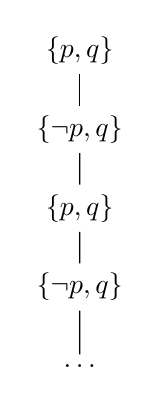
\begin{tikzpicture}
        \node {$\{p,q\}$}[level distance = 1 cm]
            child {node {$\{\neg p,q\}$}
                child{node {$\{p,q\}$}
                    child{node {$\{\neg p,q\}$}
                        child{node{$\ldots$}}
                    }
                }
            };
    \end{tikzpicture}
\end{center}

Examples of formulas which are satisfied by this word are $p\andd q$, $\X\neg p$, or the more complex 
$p\mbox{ }\andd \mbox{ }\G(q \mbox{ }\andd \mbox{ }(p \mbox{ }\orr\mbox{ } \X\neg p)\mbox{ } \andd \mbox{ }(\neg p \mbox{ }\orr\mbox{ } \X p))$, which describes exactly the nature of this model,
with $q$ always set to true and with $p$ alternating.
However, $\F(\neg p \mbox{ } \andd \mbox{ }\X\neg p)$ is not satisfied here, as we will never reach two consecutive states where 
$p$ is set to `false'.

\end{example}

\subsection{Fair CTL (Computational Tree Logic)}
CTL is a very common temporal logic, operating over infinite trees instead of infinite words.
It consists of operators such as AX (`all successors verify\ldots') and EG
(`there exists a branch where globally \ldots holds'). However, in~\cite{GhivG16}, a 
further variant named
\CTLf~was introduced, allowing to add local fairness constraints on branches. Let us define precisely
what it means.

\subsubsection*{Syntax of fair CTL}\label{subsec:syntax_CTLf}

\begin{definition}\label{CTLf_formulas}
    Let $\bar{p}= \{p_1,\ldots,p_n \}$ be a finite set of propositional variables. We define inductively 
    a \emph{$CTL^{f}$-formula} $\varphi$ to be of the shape:
    \begin{itemize}
        \setlength\itemsep{0em}
        \item[-] $\bot$
        \item[-] $p \in \bar{p}$
        \item[-] $\neg \varphi$
        \item[-] $\varphi \vee \psi$
        \item[-] $\dia \varphi$
        \item[-] $EU(\varphi,\psi)$
        \item[-] $EG(\varphi,\psi)$ 
    \end{itemize}
    For convenience, we then also define the De Morgan duals of our binary operations, respectively $\wedge$ for $\vee$; $AR$ for $EU$; $AF$ for $EG$. For the unary operator, we set $\Box \varphi = \neg \dia(\neg \varphi)$; Finally, we set $\top$ to be the negation of $\bot$, naturally.
\end{definition}

\begin{definition}\label{CTLf-algebra}
    A \emph{$CTL^f$-algebra}, is a tuple $\A=(A,\bot,\neg,\vee,\dia,EU,EG)$ which verifies each one of the following axioms:
    \begin{enumerate}
        \setlength\itemsep{0em}
        \item Boolean algebra axioms for $\vee,\neg,\bot$;
        \item Unary operator $\dia$ preserves finite joins, including the empty join $\bot$;
        \item $\dia \top = \top$;
        \item Binary operators $EU$ and $EG$ satisfy the following \emph{fixpoint axioms} for all $a,b,c$:
        \begin{itemize}
            \item[-] $a \vee (b \wedge \dia EU(a,b)) \leq EU(a,b)$
            \item[-] $a \vee (b \wedge \dia c) \leq c \implies EU(a,b) \leq c$ 
            \item[-] $EG(a,b)\leq a\wedge \dia EU(b\wedge EG(a,b),a)$
            \item[-] $c\leq a\wedge \dia EU(b\wedge c,a) \implies c \leq EG(a,b)$
        \end{itemize}
        In other words, $EU(a,b)$ is the \emph{least pre-fixpoint} of the function $x \mapsto a \vee (b \wedge \dia x)$.
        And $EG(a,b)$ is the \emph{greatest post-fixpoint} of the function $x \mapsto a\wedge \dia EU(b\wedge x,a)$.
    \end{enumerate}
\end{definition}

Importantly, we remark that for all $a,b$, $AR(a,b)$ is the greatest post-fixpoint of $x \mapsto a \wedge (b \vee \Box x)$, while $AF(a,b)$ is the least pre-fixpoint of $x \mapsto a \vee \Box AR(b\vee c,a)$.

Once again, the algebraic structure we define corresponds to what we expect of a syntax. That is, there are \emph{equations} (equalities) which correspond to axioms of a deduction system, like: \AxiomC{}\UnaryInfC{$\top\vdash\dia\top$} \[\DisplayProof\]
But there also are \emph{quasi-equations} (implications) which translate to deduction rules: \AxiomC{$c\vdash a\wedge \dia EU(b\wedge c,a)$}\UnaryInfC{$c \vdash EG(a,b)$}\[\DisplayProof\]
However, we rarely (or never) use the rules properly speaking, but we define a structure which embodies those properties and use operations on it. This is sometimes called \emph{algebraic semantics}.


Also, note that the axioms on EU and EG show that \CTLf~is a fragment of the modal \emph{$\mu$-calculus}, 
see \cite[Section 2]{SantoMu}. For example, for every $a,b$, $EU(a,b)$ can be defined as 
$\mu x.(a \vee (b \wedge \dia x))$, the least fixpoint of this monotone function (it is enough to say the least \emph{pre-fixpoint}, 
for reasons similar to those we gave for LTL. As for EG, it is a greatest \emph{(post-)} fixpoint, 
so it could have been defined with a $\nu$ operator, where $\nu f = \neg\mu(\neg f) $. 
More precisely: \[EG(a,b)=\nu y.(a\wedge\dia\mu x.((b\wedge y)\vee(a\wedge\dia x))).\] 
This makes apparent a nesting of a $\mu$ operator inside a $\nu$ operator. This is what makes the logic hard to analyse, 
compared to LTL which only contains one fixpoint operator, without alternations of $\mu$ and $\nu$.  

\begin{definition}\label{interp_form_algebra}
    For any finite set of propositional variables $\bar{p}$ and any $CTL^f$-algebra $\A$, we can define a \emph{valuation} 
    $V:\bar{p}\to A$. Then any $CTL^f$-formula $\varphi$ with variables in $\bar{p}$ can be interpreted as a term in $\A$ (the \emph{interpretation} of $\varphi$ under $V$, $\varphi^\A(V)$).

    Then, we can say the equality $\varphi(\bar{p})=\psi(\bar{p})$ is \emph{valid} if it is true under every valuation to every $A$.

    $\varphi$ and $\psi $ are said to be \emph{equivalent} if the equation $\varphi = \psi$ is valid. $\varphi$ is called a \emph{tautology} if it is equivalent to $\top$, and is said to be \emph{consistent} if it is not equivalent to $\bot$.

    Finally, we say $\varphi$ \emph{entails} $\psi$ if $\neg \varphi \vee \psi$ is a tautology, which we will denote $\varphi \vdash \psi$.
\end{definition}

\subsubsection*{Semantics of fair CTL}\label{subsec:sem_CTLf}
\begin{definition}\label{forcing_rel_CTLf}
    We first define the notion of \emph{transition system}, i.e.\ a pair $(S,R)$, where $S$ is a set, and $R$ a binary relation on $S$. 
    Then, an \emph{$R$-path} is a (possibly infinite) sequence of nodes in $S$ such that $s_i R s_{i+1}$ for all $i$. 
    Finally, for a finite set $\bar{p}$ of variables, define a \emph{$\bar{p}$-coloring} $\sigma : S \to \mathcal{P}(\bar{p})$ as above.

    We can define the forcing relation $\models$ between nodes in $S$ and formulas $\varphi$ with variables in $\bar{p}$, by induction on $\varphi$:
    \begin{itemize}
        \setlength\itemsep{0em}
        \item[-] propositional cases are defined identically as in LTL;
        \item[-] $s\models \dia\varphi$ if there exists $s'$ such that $sRs'$ and $s'\models \varphi$;
        \item[-] $s\models EU(\varphi,\psi)$ if there exists $n\geq 0$ and a path $s_0Rs_1R\ldots Rs_n$ ($s_0=s$) such that $s_k\models\psi$ for every $k<n$ and $s_n\models\varphi$;
        \item[-] $s\models EG(\varphi,\psi)$ if there exists an infinite path $s_0Rs_1R\ldots $ ($s_0=s$) such that $s_k\models\varphi$ for every $k$ and $s_j\models\psi$ infinitely often on the path.       
    \end{itemize}

\end{definition}

Note that as a consequence, $s\models\Box\varphi$ if and only if for every successor $s'$ of $s$ by $R$, $s'\models\varphi$ holds.
Also, $s\models AR(\varphi,\psi)$ if and only if for every $n\geq 0$ and every path $s=s_0Rs_1R\ldots Rs_n$, either $s_k\models\psi$ for some $k<n$, or $s_n\models\varphi$.

Similarly, $s\models AF(\varphi,\psi)$ if and only if for all infinite paths ${(s)}_k$ starting from $s_0$, if $s_j\not\models\psi$ infinitely often, then $s_k\models\varphi$ for some $k$.

Also, as a convention, we will require the transition systems to be \emph{serial}, i.e.~that every node has a successor. Syntactically, this is represented by the axiom $\dia\top = \top$.

\section{Completeness of LTL}\label{SecLTLcomp}
 
Once syntax and semantics of a particular logic are defined, the goal is to prove that the formulas they define to be true are the same,
in order for a computer system to use it and be trusted. The first part is to prove that the syntactical (or logical) system is \emph{sound}
with regard to the semantics, i.e. that every formula which can derived to be a \emph{tautology} (equivalent to $\top$) in the system is actually \emph{valid}
(true under every valuation) semantically. Soundness is usually proved by induction, examining the last rule of inference used to derive the tautology.

Completeness is the reciprocal implication, and proving it can be much harder. In the cases which are of interest to us, completeness is proved by solving the 
\emph{SAT problem}, which is the question of whether a formula has a model (is satisfiable by a valuation). Indeed, the following are equivalent:
\begin{equation*}
    \begin{gathered}
        \forall\phii (\phii\mbox{ is valid }\Rightarrow \phii\equiv\top)\\
        \forall\phii (\mbox{not(}\phii\equiv\top\mbox{)}\Rightarrow \phii\mbox{ is not valid})\\
        \forall\phii (\neg\phii\not\equiv\bot\Rightarrow \neg\phii\mbox{ is satisfiable})\\
        \forall\psi (\psi\not\equiv\bot\Rightarrow \psi\mbox{ is satisfiable}) \\
    \end{gathered}
\end{equation*}
 
Then it is sufficient to show that every \emph{consistent} formula (not equivalent to $\bot$) is satisfiable.

This is why this section will focus on the different ways the SAT problem is handled in LTL. In the literature, we distinguish between two
major families of approaches: automata- and tableaux- based. We will go at length about the major assets and setbacks of both approaches.

\subsection{Automata for LTL}

The approch we will describe comes from F. Laroussinie's MPRI course (\cite[pages 22-36]{LarouLTL}); variants can be found in \cite[Section 3]{CristauAuto},
\cite[Section 1.3]{GastinAuto}. Also look at this \href{http://www.lsv.fr/~gastin/ltl2ba/index.php}{implementation in C}, computing accepting Büchi automata for LTL
formulas (presented in \cite[Pages 53-65]{OddouxProg}).
    
- DESCRIBE AT LENGTH ONE AUTOMATA-BASED ALGO FOR LTL SAT (EX LAROUSSINIE) + CITE OTHERS

\subsection{Tableaux for LTL}

- DESCRIBE A TABLEAU METHOD, A CLASSIC INVOLVING GRAPHS (EX WOLPER) + CITE OTHERS

- TRANSITION : ONE LAST EXAMPLE WHICH WE WILL TREAT IN THE FOLLOWING SECTION

\section{Reynolds' SAT Solver for LTL: an implementation}\label{SecOcaml}

Reynolds' tableaux algorithm~(\cite{ReyLTL}, 2016) for LTL, unlike other methods based around automata, was conceived
with implementation in mind. In the abstract, the author claims that his tree-style tableau is simple to understand, which we will
certainly agree on: rules are designed in the most straightforward way, and the visuals are immediate to get. This quickly lead us 
to study the algorithm, and what was conceived like a practical experimentation of the method quickly became a large part of this internship.

The greatest feature of this paper is to use trees (instead of automata, or graphs used by classic tableaux), which allows to
make the most benefit out of recursion, not having to create massive data structures. We will briefly describe the algorithm, before discussing
more precisely the details of our implementation in OCaml. Note once again that we restrict the language to unary LTL,
that is, LTL without `Until'.


\subsection{Reynolds' tableaux algorithm for LTL}

We will write the algorithm in pseudo-code, then explain the most important parts of it.\\

{\tt 

Input: Unary-LTL formula $\phii$

Select any order of exploration of the leaves

Set S $\gets$ $\{\phii\}$

Tree T $\gets$ Root labeled S

While (There is at least one uncrossed leaf):

\hspace*{1cm} S $\gets$ Next uncrossed leaf in the order

\hspace*{1cm}   If S is empty:

\hspace*{1cm}\hspace*{1cm}    Return True

\hspace*{1cm}    Else if S contains $\bot$ :
    
\hspace*{1cm}\hspace*{1cm}        Cross leaf
        
\hspace*{1cm}\hspace*{1cm}       S$\gets$next uncrossed leaf if there is one

\hspace*{1cm}    Else if S contains two contradictory formulas $\psi$ and $\neg\psi$:

\hspace*{1cm}\hspace*{1cm}      Cross leaf
        
\hspace*{1cm}\hspace*{1cm}      S$\gets$next uncrossed leaf if there is one

\hspace*{1cm}    Else if a unary static rule applies:

\hspace*{1cm}\hspace*{1cm}      S'$\gets$S updated along rule

\hspace*{1cm}\hspace*{1cm}       Add leaf labeled S' below S

\hspace*{1cm}    Else if a binary static rule applies:

\hspace*{1cm}\hspace*{1cm}       S1$\gets$S updated along rule case 1

\hspace*{1cm}\hspace*{1cm}        S1$\gets$S updated along rule case 2
        
\hspace*{1cm}\hspace*{1cm}        Add two leaves labeled S1, S2 below S

\hspace*{1cm}    Else if LOOP Rule applies:

\hspace*{1cm}\hspace*{1cm}      Return True

\hspace*{1cm}   Else if PRUNE Rule applies:

\hspace*{1cm}\hspace*{1cm}      S$\gets$next uncrossed leaf if there is one

\hspace*{1cm}   Else if {PRUNE}$_0$ Rule applies:

\hspace*{1cm}\hspace*{1cm}       S$\gets$next uncrossed leaf if there is one

\hspace*{1cm}   Else:

\hspace*{1cm}\hspace*{1cm}      S'$\gets$S updated along TRANSITION Rule

\hspace*{1cm}\hspace*{1cm}      Add leaf labeled S' below S

Return False \newline

}

Most static rules are straightforward, so we will only specify a few: 
\begin{itemize}
    \item [-] if a set contains some formula of the form $\psi\andd\chi$, it is replaced by both $\psi$ and $\chi$;
    \item [-] any $\neg\neg\psi$ in a set is replaced by $\psi$;
    \item [-] if a set contains some $\neg\G\psi$, the tree forks into two cases, one with the formula replaced by $\neg\psi$, the
    other with $\X\neg\G\psi$.
    \item [-] etc.
\end{itemize}

The most innovative part of the algorithm are the `dynamic rules': LOOP, PRUNE, {PRUNE}$_0$, TRANSITION.

TRANSITION is the rule we apply to a leaf when nothing else is possible, meaning that we have simplified a set of formulas the most we could. It gets 
rid of literals (formulas of the form $p$ or $\neg p$), which describe the valuation of the node in the model being constructed; then,
it takes the remaining formulas in the set labeling the leaf, which all are of the form $\X\psi$ or $\neg\X\psi$, and removes the `Next' operator,
meaning that we have moved onto the next state.

LOOP, PRUNE (and {PRUNE}$_0$, which is a variant of PRUNE) are the rules which decide what happens when a branch becomes periodic without ever 
coming to a conclusion.

Let us talk specifically of PRUNE.
We will state the rule as it is in Reynolds' paper (\cite{ReyLTL}), then explain its meaning; reasoning about the other rules is similar.

\begin{definition}
    \emph{(PRUNE rule)}
    Suppose that $u < v < w$ and each of $u$, $v$ and $w$ have the same poised
    label $\Gamma$. Suppose also that for each $\X$-eventuality of the form $\X\F\beta$ in $\Gamma$, if there is $x$ with
    $\beta \in \Gamma_x$ and $v < x \leq w$ then there is $y$ such that $\beta\in\Gamma_y$ and $u < y \leq v$. Then $w$ can be a
    crossed leaf.
\end{definition}

\begin{center} 
    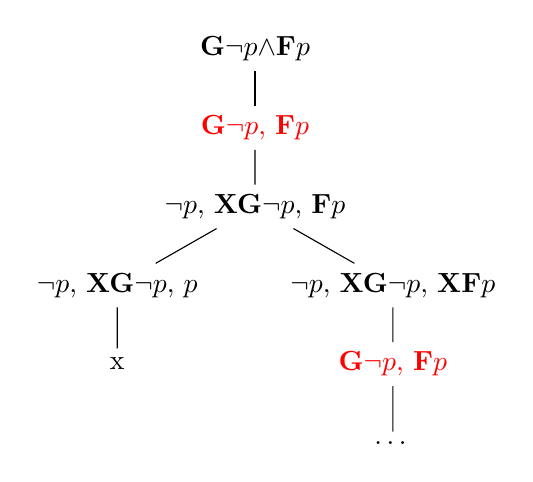
\begin{tikzpicture}
        \node {$\G\neg p\andd \F p$}[level distance = 1 cm]
            child {node[red] {$\G\neg p$, $\F p$}
                child{node {$\neg p$, $\X\G\neg p$, $\F p$}[sibling distance = 3.5cm]
                    child{node{$\neg p$, $\X\G\neg p$, $p$}
                        child{node {x}}
                    }
                    child{node{$\neg p$, $\X\G\neg p$, $\X\F p$}
                        child{node[red] {$\G\neg p$, $\F p$}
                            child{node{\ldots}}
                        }
                    }
                }
            };
    \end{tikzpicture}
\end{center}

In the example above, we can see that the tree periodically loops into the same state labeled by the set $\{\G\neg p$, $\F p\}$;
however, the $\X$-eventuality $\F p$ is never fulfilled, as the left branch is discarded by the contradiction rule. The PRUNE rule
makes sure that when formulas of the type $\F\psi$ are postponed indefinitely, the branch is discarded for not making any progress.

\subsection{An implementation in OCaml}

We recall once again that the following project can be found 
\href{https://github.com/anatcaramba/LTL-SAT-Solver-by-Reynolds-Tableaux}{here},
where more information is available about prerequisites, execution, etc.

\subsubsection*{Why OCaml?}
The choice of a functional programming language was guided by the close relationship
between inductive definitions of the formulas and the pattern matching feature.
Throughout the program, functions make use of matching, both to discriminate
what we call `eventuality formulas' from others, and to construct a printer
for LTL formulas, delving into the possible imbrications of operators to construct
a readable string.

Recursivity has proven to be an important feature to program the tableaux algorithm. 
As we will get into below, the recursive structure of the satisfiability function,
constructed as a tree, is efficient. It also makes use of the way logical disjunction
is evaluated in OCaml: we want to algorithm to stop as soon as a branch is validated,
not looking at the unfinished ones. This is exactly what disjunction does in OCaml.

Functional programming also comes with its setbacks. A quite unoptimized section of 
the program is loop checking (LOOP and PRUNE rules). We need to check a condition on 
elements in the list between two indexes. Unlike in an imperative language, accessing
a specific element in a list is not immediate. 

Another issue arises with the LOOP rule. As objects 
are immutable, we could not find an efficient way to compute a model when a branch is
validated thanks to LOOP. 

Note that the following implementation is a \emph{prototype}, and its aspect is 
experimental rather than optimized. In contrast, Leviathan (\cite{Leviathan})
is an implementation of the algorithm in \CC, which was developed by a group of researchers including Mark Reynolds;
it is much more complete than was is presented below, making use of parsers for inputs,
telling users where to loop to find infinite models, etc. The tool can be downloaded on \href{https://github.com/Corralx/leviathan}{this webpage}.
In the same vein, `BLACK'~\cite{Black21} is more recent and incorporates SAT solvers.
    
\subsubsection*{Overview of the implementation}

Most of the program uses the newly defined {\tt ltl} type, which is based on the inductive 
definition of LTL formulas we have given, and will allow to apply recursion nicely.
Note again that we do not use operator Until.
\begin{lstlisting}
type ltl =
| Prop of char
| Top
| Bot
| Neg of ltl
| And of ltl * ltl
| Or of ltl * ltl
| F of ltl
| G of ltl
| X of ltl
\end{lstlisting}

Type {\tt ltl$\_$op} is an additional tool to characterize an LTL function by its main operator.
The program contains a handful of useful functions such as {\tt contains$\_$contra}, {\tt belongs$\_$list}
or {\tt are$\_$equal}, which often are not much more than tools made out of the original librairies
of OCaml (List, mainly).

We have chosen to view a node of the tableau as a {\tt ltl list list}.
First of all, it makes perfect sense for a
node to be represented as a {\tt ltl list}, given that the algorithm unravels the subformulas which 
have to be satisfied if the formula has to be true. Then, we need to be able to keep trace
of ancestors of every node, in case we need to check if rules LOOP, PRUNE, PRUNE$_0$ apply.
However, since OCaml deals with immutable objects, it was not obvious to us how to create a global tree structure
that we would update throughout the algorithm. Then the easiest way to deal with this was
to pass the ancestors as parameters
in our recursive process. This is why we treat every node as a {\tt ltl list list}. A potential future improvement 
would be to actually create this tree structure.

Main function {\tt sat} is given in the appendix; it has no innovative feature, and mostly
follows 
the structure of Reynolds' algorithm (\cite{ReyLTL}). In addition to that, it prints 
the unravelling of the tree, namely: specify which formulas are to be satisfied 
in each node, tell when there is branching, when a branch is discarded or validated and why.
We tried to give the main information while keeping the output readable.

The most intricate functions in the program are those designed to test `dynamic'
termination rules: LOOP, PRUNE and PRUNE$_0$. For example, take the LOOP rule as defined in 
\cite{ReyLTL}. 
\begin{definition}
    \emph{(LOOP rule)}
    If a node $v$ with poised label $\Gamma_v$ has a proper ancestor (i.e. not itself) $u$ with
poised label $\Gamma_u$ u such that $\Gamma_v \subseteq \Gamma_u$, and such that for each $\X$-eventuality of the form $\X\F\beta$ in $\Gamma_u$ we
have a node $w$ such that $u < w \leq v $ and $\beta \in$ $\Gamma_w$ then $v$ can be a validated leaf.
\end{definition}
Here is our function, which returns true if and only if the LOOP rule
applies to the tableau.
\begin{lstlisting}
let loop_applies (ll:ltl list list):bool=
    let i = poised_ancestors_contain ll in
        let current_list = List.hd ll in
            List.exists(fun k_v -> is_included (List.nth ll k_v)(current_list) &&
(* there is a proper poised ancestor v contained in current poised label and *)
                List.for_all(fun phi->List.exists (fun j->belongs_list phi (List.nth ll j)) (range 1 (k_v+1) ))(f_X_ev (current_list)))i
(* every XF-ev in current label was satisfied after v *)
\end{lstlisting}

The {\tt List.exists} and {\tt List.for$\_$all} imbrication (lines 4 to 8), while not immediate to read, is a rewriting 
of the sentence in LOOP rule. However, the subtlety is that {\tt poised$\_$ancestors$\_$contain}, given the current unraveling
of the tableau {\tt ll}, returns a list of \emph{integers}, that is, the indices of the current node's poised ancestors
which contain the current node. This points to the set of nodes named $u$ in the above definition. Then, tests such as 
{\tt List.exists} access the actual poised label $\Gamma_u$ with {\tt List.nth}. This solution is unoptimized, as in OCaml 
this access takes linear time in the most general case (and not constant, as it would in C). 
A future improvement would be to track poised ancestors in a global structure,
so that the program does not compute the same list of ancestors twice. At this point, it appears clearly that 
the algorithm takes benefit from both functional- and object- oriented programming features. 

As we hinted towards earlier in this section, 
we did not yet manage to give a precise model when satisfiability is proved thanks to the LOOP rule. The program simply tells 
to `loop from here', but whether to repeat the last state indefinitely, or the last two, three or more
states is left to the user.
While the answer should not be too far-fetched in usual cases, one can easily imagine a large-sized model where 
the user could not do without advice. What prevents us to find the answer for now is, again, the nature 
of the {\tt loop$\_$applies} function. {\tt List.exists}\ldots $\mbox{ }$ returns {\tt true} if an ancestor meets the right conditions,
but not its index. So computation of models would also benefit from a global structure for the tree,
keeping all necessary information
in memory. 

\subsubsection*{Performance}
Among a battery of tests, we have created a sequence of formulas that exhibits the worst-case performance of the solver. 
It corresponds to the `exponential case' test. This sequence of `worst-case formulas' 
is built by taking {\tt Bot} at rank 0 (or any unsatisfiable formula), and out of rank n, 
build rank n+1 by taking the disjunction of two times the formula at rank n. 
The formula in the test case only has rank 5, however we have tested up to 13 nestings. 
Since the procedure is PSPACE-complete (see \cite[Section 9]{ReyLTL}), 
we would expect an exponential time in function of the number of nestings in the worst case, 
which is what we seem to get. 

\begin{figure}[h!]\label{fig:graph_perf}
    \centering
    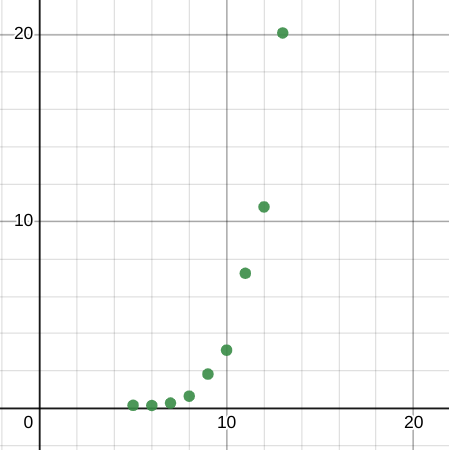
\includegraphics[width = 4cm]{graph_perf.png}
    \caption{Evolution of the `exponential case' test with the depth of nestings.}
\end{figure}
\begin{table}[h!]
    \centering
    \begin{tabular}{|l|l|l|l|l|l|l|l|l|l|}
    \hline
    Number of nestings & 5    & 6    & 7    & 8    & 9    & 10   & 11   & 12    & 13    \\ \hline
    Testing time (s)   & 0.17 & 0.16 & 0.29 & 0.66 & 1.84 & 3.12 & 7.23 & 10.78 & 20.08 \\ \hline
    \end{tabular}
\end{table}




This is normal, as adding a nesting doubles the number of leaves, 
all of which end up crossed (so the algorithm has to check every one of them).

\subsubsection*{Future improvements}
\begin{itemize}
    \item [-] Upgrade the main function with global objects, keeping track of information invariant throughout the computation of a model. This would make the implementation faster, as well as compute precise models in the case they loop from a number of states. Also, there is no evidence that a large number of recursions does not saturate the space allowed by memory.
    \item [-] Implement parsers to make the program more user-friendly. Rather than having to go through the top-level, the user should be able to execute the function directly in a terminal, with a tolerance for different syntaxes of formulas. The issue for now is being able to transcript a string into an actual {\tt ltl}-typed object.
    \item [-] The chosen syntax makes it hard for longer formulas to be both read, and typed by hand. For user-comfort purposes, and to allow tests on formulas which could really reach the program's limit, we should be able to write scripts that automatically generate formulas.
\end{itemize}


\section{Towards a constructive proof for completeness of fair CTL}\label{SecCTLfcomp}

\subsection*{Problem}
The multitude of approaches that exist for proving LTL completeness inclines us to do adapt them to more complex temporal logics,
and \CTLf~in particular. Once again, our main concern is the actual computation of models. In other words, the question is
whether we can find an answer to the SAT problem for \CTLf~which is \emph{constructive}; we would like to write an algorithm 
which tells us, for a \CTLf-formula $\phii$, a transition system $(S,R)$ and a finite set of variables $\bar{p}$, which $\bar{p}$-coloring 
$\sigma : S \to \mathcal{P}(\bar{p})$ (or even better, which set of colorings) of $S$ satisfies $\phii$.

As we can recall from section \ref*{SecIntro}, both binary operators EG and EU could have been defined in terms of
modal $\mu$-calculus. In particular: \[EG(a,b)=\nu y.(a\wedge\dia\mu x.((b\wedge y)\vee(a\wedge\dia x))).\]
The nesting of a \emph{least pre-fixpoint operator} ($\mu$) inside a \emph{greatest post-fixpoint operator} ($\nu$)
is what makes the completeness proof of \CTLf~more than just an update from that of LTL. In the latter, the only `eventuality' operator is $\F$, which
we could have defined as \[\forall a, \F a = \mu x. (a\orr\X\F x)\] Looking back at Reynolds' algorithm, testing satisfiability
of $\F\phii$ amounts to checking if $\phii$ can be satisfied, and if not, test $\F\phii$ in the next state, concluding negatively if 
the branch just loops without ever satisfying $\phii$. This is because $\F$ is \emph{constructive}.

\subsection*{Constructive operators in fair CTL}

We define, given a transition system $(S,R)$, a \CTLf-algebra which we consider canonic for the system, i.e. which transcripts in algebraic
terms the definitions we gave in section \ref*{SecIntro} for semantics for \CTLf~(see \cite[Section 2]{GhivG16}).

\begin{definition}\label{complex_algebra}
    Given a transition system $(S,R)$, its \emph{complex algebra} is the tuple \[\mathbb{P}_{(S,R)}=(\mathcal{P}(S),\emptyset,S\backslash(-),\cup,\diamond_R,EU_R,EG_R)\] which is the classical Boolean algebra over the powerset of $S$, along with operators \[\diamond_R(a)=R^{-1}[a]=\{s\in S \mid \exists t\in a, sRt \}\] and $EU_R$ and $EG_R$ defined as fixpoints (see above) so that we finally have a $CTL^f$-algebra. 
\end{definition}

Now, completeness becomes equivalent to proving that for every \CTLf-formula $\phii$ with variables in $\bar{p}$, 
if there exists a satisfying interpretation of $\phii$ in $\mathbb{P}_{(S,R)}$, then there exists one in every \CTLf-algebra $A$.

Indeed, $\mathbb{P}_{(S,R)}$ is designed so that 
a \CTLf-formula $\phii$ is semantically true if and only if there exists an interpretation of $\phii$ in $\mathbb{P}_{(S,R)}$ which satisfies $\phii$.
This is almost obvious from definitions for propositional cases and $\diamond$; for EU and EG, we use the following lemmas:

\begin{lemma}\label{EU_as_union}
        For every $a,b$ in $\mathbb{P}_{(S,R)}$ it holds that \[EU_R(a,b)=\bigcup_{i=0}^{\infty}D_n(a,b)\] where $D_n$ is defined inductively as
        \begin{equation*}
            \begin{cases}
                D_0(a,b)=\emptyset\\
                D_{n+1}(a,b)=a\cup(b\cap\diamond_R D_n(a,b))
            \end{cases}
        \end{equation*}
        
\end{lemma}

\begin{proof}
    \begin{itemize}
        \item[$\supseteq$] By induction on n we show $D_n(a,b) \subseteq EU_R(a,b)$.
        \item[$\subseteq$] We show that $D(a,b) := \bigcup_{i=1}^{\infty}D_n(a,b)$ is a pre-fixpoint of $x \mapsto a \cup (b \cap \diamond x)$. From the definition of $EU$ the inclusion directly follow.
    \end{itemize}
\end{proof}

We can now state the corresponding lemma for $EG$:
\begin{lemma}\label{EG_as_set}
    For every $a,b$ in $\mathbb{P}_{(S,R)}$ it holds that $EG_R(a,b)$ is the set:
\begin{multline*}
    \{s\in S\mid \mbox{there exists an infinite path } s=s_0Rs_1R\ldots\\
    \mbox{ such that }\forall k\in \mathbb{N} \mbox{ } s_k\in a\mbox{, and } s_{j}\in b \mbox{ for infinitely many } j \in\mathbb{N}\}
\end{multline*}
\end{lemma}

Operator $EU$ is \emph{constructive} (see~\cite[Intro]{SantoMu}), because it can be described using pre-existing operators of the syntax; whereas the concept of `infinite path' introduced by operator $EG$ cannot be reduced to anything else, so $EG$ is not constructive. In particular, we do \emph{not} have the equality: \[EG_R(a,b)=\bigcap_{i=1}^\infty D'_n(a,b)\] where
\begin{equation*}
    \begin{cases}
        D'_0(a,b)=\mathcal{P}(S)\\
        D'_{n+1}(a,b)=a\cap\diamond_R EU_R(b\cap D'_n(a,b),a)
    \end{cases}
\end{equation*}
Although the analogy is pretty clear (the sets are defined as an sequence induced by the `fixpoint function' of the operator), it doesn't work because it fails to grasp infinite paths. For example, we can construct a tree belonging to every $D'_n(a,b)$ (for every $n$ there is a finite path where every node is in $a$, and $b$ contains at least $n$ nodes), but such that no infinite path has the wanted property (of belonging to the set described in the last lemma). Informally, the following infinite binary tree is in every $D'_n(\mathcal{P}(S),b)$ but not in $EG_R(\mathcal{P}(S),b)$:
\begin{center} 
\begin{tikzpicture}
        \node {$\neg b$}[sibling distance = 2.5cm][level distance = 1 cm]
            child {node [red]{$b$}[sibling distance = 1cm]
                child{node {$\neg b$}[sibling distance = 1cm]}
                child{node {$\neg b$}[sibling distance = 2.5 cm]}}
            child {node {$\neg b$} [sibling distance = 2.5cm]
                child{node[red]{$b$}[sibling distance = 1cm]
                    child {node [red]{$b$}[sibling distance = 1cm]
                        child {node {$\neg b$}[sibling distance = 1cm]}
                        child {node {$\neg b$}[sibling distance = 2.5cm]}}
                    child {node {$\neg b$}[sibling distance = 2.5cm]}}
                child{node {$\neg b$}[sibling distance = 2.5cm]
                    child {node [red]{$b$}[sibling distance = 1cm]
                        child{node [red]{$b$}[sibling distance = 1cm]
                            child {node [red]{$b$}[sibling distance = 1cm]
                                child {node {$\neg b$}[sibling distance = 1cm]}
                                child {node {$\neg b$}[sibling distance = 2.5cm]}}
                            child {node {$\neg b$}[sibling distance = 2.5cm]}}
                        child {node {$\neg b$}[sibling distance = 2.5cm]}}
                    child {node {$\neg b$}[sibling distance = 2.5cm]
                        child{node{...}}
                        child{node{...}}}}};
    \end{tikzpicture}
\end{center}


\subsection*{Ultrafilter computation}

The proof of completeness for \CTLf~in~\cite[Section 3]{GhivG16} uses tableaux, but does not provide a way to compute a model for satisfiable formulas.
The idea the proof starts with is fixing a general formula $\phii_0$ which is \emph{consistent} in a \CTLf-algebra $\A$ (not equal to $\bot$).
The goal will be to prove that there exists a transition system  and a valuation satisfying $\phii_0$, therefore proving completeness. But 
the model is never \emph{actually} computed. Because $\phii_0$ is not equal to $\bot$, there exists an \emph{ultrafilter} $x_0$
in $\A$ such that $\phii_0 \in x_0$ (see~\cite[Section 3.3]{GehvG22}). From there on, the specific tableaux method is unraveled, using the 
\emph{ultrafilter frame} of $\A$; but we never really know what $x_0$ consists of, and what formulas it contains. This 
is the object of the research we present below.

\subsubsection*{Atomic lower bounds}
Not every infinite algebra is \emph{atomic}, which means that maybe not every ultrafilter in $\A$ has a minimum.
What is sure is that if there is a formula $\varphi_{0,m}$ such that $x_0 =$ $\uparrow\varphi_{0,m}$,
it must be absolutely restrictive on which trees can be accepted as models. Let us precise what this means. 
\begin{definition}\label{phi_m}
    Let $a$ be a consistent $CTL^f$-formula. We say that a formula $a_m$ is an \emph{atomic lower bound for $a$} if 
    \begin{enumerate}
        \item $\bot<a_m\leq a$
        \item for every $CTL^f$-formula $\psi$ we have either $\psi\wedge a_m=a_m$, or $\psi\wedge a_m=\bot$.
    \end{enumerate}
    Equivalently, $a_m$ is an atomic formula beneath $a$.
\end{definition}
For every $p$ in $\bar{p}$, for every $n \geq 0$, we should have either $\diamond^np \wedge \varphi_{0,m} = \varphi_{0,m}$, 
or $\diamond^np \wedge \varphi_{0,m} =\bot$. In informal terms, either all models of $\varphi_{0,m}$ contain a $n$-th successor 
for the root whose coloring contains $p$, or none of them do. The same reasoning with $\diamond^n\neg p$ leads us to say that for every $n$, 
for every $p$ in $\bar{p}$, \[\varphi_{0,m}\vdash\Box^n p\mbox{ or } \varphi_{0,m}\vdash\Box^n\neg p.\]
One way to restate this is by saying that colorings of models are determined by formula $\varphi_{0,m}$. Thus, we would like to construct this formula from $\varphi_0$ by fixing colorings which are not determined by it. An immediate problem is that formulas in the logic are finite, while trees are infinite. Even with the simplest of consistent formulas, $\varphi_0 = \top$, building $\varphi_{0,m}$ only with boxes is impossible, as there are infinitely many formulas $\bigwedge_{p\in\bar{p}}\bigwedge_{k=0}^n\Box^k p$ which are below $\top$. We need a formula which is below $\bigwedge_{p\in\bar{p}}\bigwedge_{k=0}^n\Box^k p$ for every $n$, and a fitting candidate is $\bigwedge_{p\in\bar{p}}AR(p,\bot)$, as \[AR(p,\bot)=p\wedge\Box AR(p,\bot)=p\wedge\Box p\wedge \Box AR(p,\bot)=... .\] Actually, we can define $\top_m=\bigwedge_{p\in\bar{p}}AR(p,\bot)$. 
\begin{proposition}\label{top_m}
    For every $CTL^f$ formula $\psi$, we have either $\top_m\wedge\psi=\bot$, or $\top_m\wedge\psi=\top_m$.
\end{proposition}
\begin{proof}
    We proceed by induction over the structure of $\psi$. Note that due to the structure of $\top_m$, 
    it is sufficient to show the property that for every $p\in\bar{p}$, either $\ARp\wedge\psi=\bot$ or $\ARp\wedge\psi=\ARp$.
    In this report, we will specify only one point, but readers are encouraged to check the other points by themselves.
    \begin{itemize}
        \setlength\itemsep{0em}
        \item[-] let $\phi = EU(\psi,\chi)$. Suppose that the property holds for $\psi$ and $\chi$, by induction. Let $p$ in $\bar{p}$. We first show that \[AR(p,\bot)\wedge EU(\psi,\chi)=EU(\psi\wedge AR(p,\bot),\chi\wedge AR(p,\bot))\]
            First, 
            \begin{align*}
                &EU(\psi\wedge AR(p,\bot),\chi\wedge AR(p,\bot))\\
                &=[\psi\wedge\ARp]\vee[\chi\wedge\ARp\wedge\diamond EU(\psi\wedge AR(p,\bot),\chi\wedge AR(p,\bot))]\\
                &=\ARp\wedge(\psi\vee[\chi\wedge \diamond EU(\psi\wedge AR(p,\bot),\chi\wedge AR(p,\bot))])\\
                &\leq\ARp\wedge(\psi\vee[\chi\wedge \diamond EU(\psi,\chi)])\mbox{ by monotonicity}\\
                &=\ARp\wedge EU(\psi,\chi).
            \end{align*}
            On the other hand, we will show that \[EU(\psi,\chi)\leq EU(\psi\wedge\ARp,\chi\wedge\ARp)\vee\neg\ARp.\] 
            By a least fixpoint argument using definition of $EU(\psi,\chi)$, a sufficient condition is 
            \begin{multline*}
                \psi\vee(\chi\wedge\diamond [EU(\psi\wedge\ARp,\chi\wedge\ARp)\vee\neg\ARp])\\
                \leq EU(\psi\wedge\ARp,\chi\wedge\ARp)\vee\neg\ARp.
            \end{multline*}
            Equivalently, by switching back $\ARp$ to the left side and by developing on the left, we only need to prove
            \begin{multline*}
                [\ARp\wedge(\psi\vee[\chi\wedge\diamond EU(\psi\wedge\ARp,\chi\wedge\ARp)])]\\
                \vee[\ARp\wedge\psi]\vee[\chi\wedge\ARp\wedge\diamond\neg\ARp]\\
                \leq EU(\psi\wedge\ARp,\chi\wedge\ARp)
            \end{multline*}
            As the left member simplifies, this is still equivalent to 
            \begin{multline*}
                [\ARp\wedge\psi]\vee[\ARp\wedge\chi\wedge\diamond EU(\psi\wedge\ARp,\chi\wedge\ARp)]\\
                \leq EU(\psi\wedge\ARp,\chi\wedge\ARp)
            \end{multline*}
            which is true by definition of $EU$. Therefore, the inequality is proven in both ways, which states our first equality.
            Now, by induction hypothesis, there are four cases, depending on the values of $AR(p,\bot)\wedge\psi$ and $AR(p,\bot)\wedge\chi$. In each case, it is straightforward to check that $EU(\psi\wedge AR(p,\bot),\chi\wedge AR(p,\bot))$ is either equal to $\bot$, or $AR(p,\bot)$, which concludes the proof for this point.
    \end{itemize}
\end{proof}


This definition of $\top_m$ is satisfying, and we would like to extend this construction to all literals by defining
 \[p_m:=\top_m\] \[(\neg p)_m:=AR(\neg p,\bot)\wedge\bigwedge_{q\in\bar{p},q\not=p}AR(q,\bot).\] But here is the problem: 
 while this definition for literals is the most natural from what we could guess, it does not fare well by induction. 
 We cannot define $(\varphi_0\wedge\varphi'_0)_m=\varphi_{0,m}\wedge\varphi'_{0,m}$. 
 Take for instance $\bar{p}=\{p,q\}$, $\varphi_0=p$ and $\varphi'_0=\neg q$: following the previous construction we have 
 \[\varphi_{0,m}\wedge\varphi'_{0,m}=AR(p,\bot)\wedge AR(q,\bot)\wedge AR(\neg q,\bot)=\bot.\]

This is why we stopped here in our search for atomic lower bounds of \CTLf~formulas. However, using automata to compute
the set of \emph{all} atoms beneath $\phii_0$ might be the next step towards actually computing ultrafilters, or finding another
constructive solution to the SAT problem for \CTLf. This is left to future work.


\section*{Acknowledgments}
    I would like to thank Adrien Guatto of IRIF for his advice on the implementation in OCaml, and the FSMP for
    financing this internship. Most of all, I am grateful for my supervisor's availability, insight and support 
    during these five months.
\bibliography{bibli}
\end{document}